\documentclass[12pt]{article}

\usepackage[margin=0.8 in]{geometry}
\usepackage{amsmath}
\usepackage{amssymb}
\usepackage{mathtools}
\usepackage{enumerate}
\usepackage{verbatim}
\usepackage{amsthm}
\usepackage{hyperref}

\title{}
%\content{}



\let \proj \undefined
\newcommand{\p}{\partial}
\newcommand{\R}{ \mathbb{R}}

\DeclareMathOperator{\proj}{proj}
\newcommand{\sS}{\mathscr{S}}
\DeclareMathOperator{\comp}{comp}
\newcommand{\A}{\mathcal{A}}
\newcommand{\D}{\mathcal{D}}
\newcommand{\e}{\epsilon}
\newcommand{\et}{\tilde{\e}}
\newcommand{\vr}{\vec{r}{}}
\newcommand{\vF}{\vec{F}}
\newcommand{\triple}{\iiint_E f(x,y,z)dV}
\renewcommand{\lg}{\langle}
\newcommand{\rg}{\rangle}
\newcommand{\Q}{\frac{\p Q}{\p x}}
\renewcommand{\P}{\frac{\p P}{\p y}}
\let\implies\Rightarrow
\newcommand{\px}{\frac{\p}{\p x}}
\newcommand{\py}{\frac{\p}{\p y}}
\newcommand{\Fline}{\vF\cdot d\vr}


\newenvironment{solution}
  {\begin{proof}[Solution]}
  {\end{proof}
  
  }
\newtheorem{example}{Example}
\newtheorem{exercise}{Exercise}
\newtheorem{theorem}{Theorem}
\newtheorem{definition}{Definition}


\begin{document}
\section*{Green's Theorem	}
What to know
\begin{enumerate}
\item Be able to state Green's theorem
\item Be able to use Green's theorem to compute line integrals over closed curves
\item Be able to use Green's theorem to compute areas by computing a line integral instead
\item From the last section (marked with *) you are expected to realize that Green's theorem doesn't apply if the functions $P$, $Q$ involved are singular in the domain. I would strongly recommend studying this example, but I will not ask you to repeat it in an exam.
\end{enumerate}

As you saw in your first calculus courses, the Fundamental Theorem of Calculus relates the integral of the derivative of a function on an interval with its values on the boundary. In this section we will generalize the Fundamental Theorem of Calculus in $2$ dimensions.

We'll use a positively oriented simple closed curve in $\R^2$. What those words mean:
\begin{itemize}
\item \textbf{Closed:} it starts and ends at the same point
\item \textbf{Simple:} It doesn't intersect itself
\item \textbf{Positively oriented:} (for simple closed curves) transversed in counterclockwise direction
\end{itemize}

\begin{figure}[h]
\begin{center}
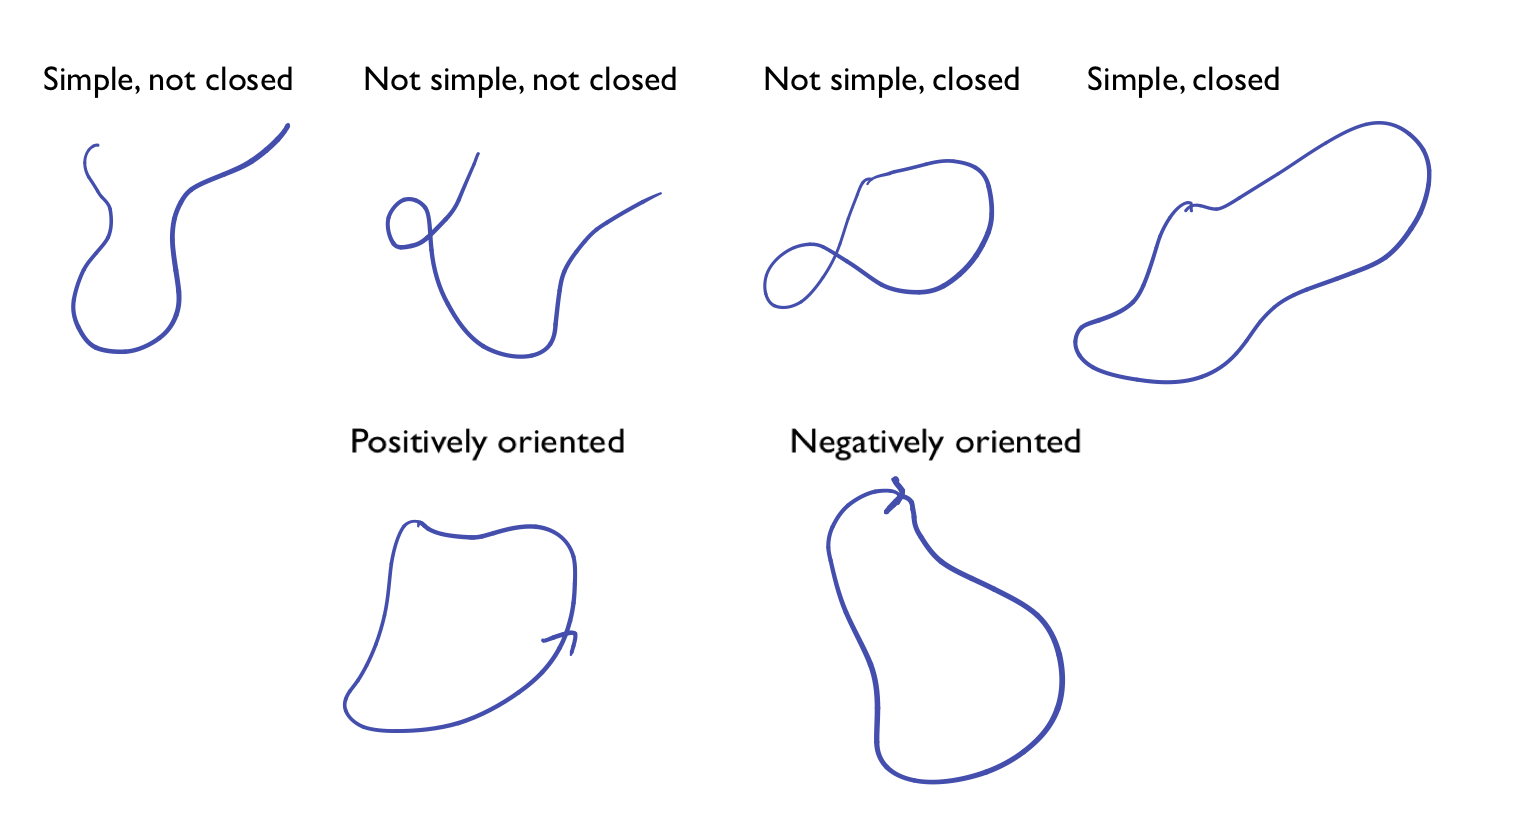
\includegraphics[scale=.3]{definitions.jpeg}
\end{center}
\end{figure}

It took mathematicians many years and many failed attempts to prove that a simple closed curve divides the plane into exactly two sets, one bounded and one unbounded (this result is called Jordan curve theorem). You can find some cool pictures of simple closed curves here: \url{http://www.dominoartwork.com/tspart.html}.

\begin{theorem}(Green's)
Let $c$ be a simple, closed and positively oriented piecewise smooth curve, let $D$ be the bounded domain enclosed by $c$ and assume that $\vF=\lg P,Q\rg$ is a vector field such that $P$ and $Q$ are \textbf{everywhere continuously differentiable on $D$}. Then
\begin{equation}
\int_c\vF\cdot d\vr=\int_cPdx+Q dy=\int_D\left( \Q-\P\right )dA
\end{equation}
\end{theorem}

\begin{figure}[h]
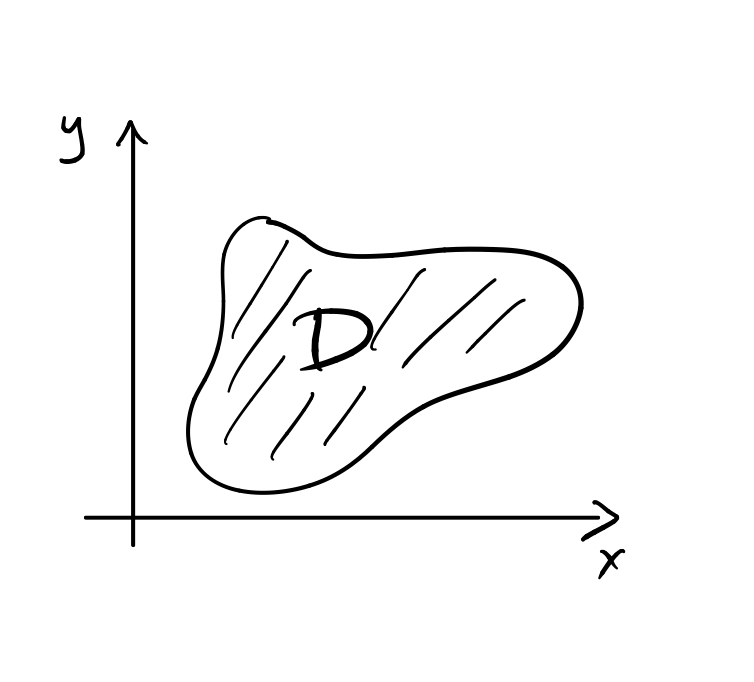
\includegraphics[scale=.3]{thm.jpg}
\end{figure}


\textbf{Remarks:}
\begin{itemize}
\item Recall from an earlier section that $\int_{-c}\vF\cdot d\vr=-\int_c\vF\cdot d\vr$. Therefore, if $c$ is a \textbf{negatively oriented} simple, closed piecewise smooth curve, $$\int_c\vF\cdot d\vr=-\int_D\left( \Q-\P\right )dA.$$
\item If $\vF$ is conservative, as we saw in last section, it satisfies $\P=\Q$, so Green's theorem implies $\int_c \vF \cdot d\vr=0 $ over a simple closed curve (as expected).
\end{itemize}

So why do we care about Green's theorem? The FTC for intervals was useful to calculate an integral over the interval, but here things are reversed in a sense. Green's theorem is most useful for \textbf{calculating line integrals of vector fields over closed paths and it should be your first thought when you need to calculate one}. It's usually not that useful for double integrals, since if you have to compute $\iint_D f dA $ you'd need to write $f=\P-\Q$. There is one notable exception to this, when we use Green's theorem to find the area of a domain, see below.

\begin{example}
Compute $\int_c xy^2dx +2x^2 y dy$, where $c$ is the positively oriented triangle with vertices $(0,0)$, $(2,2)$ and $(2,4)$.
\end{example}
\begin{solution}
\begin{figure}[h]
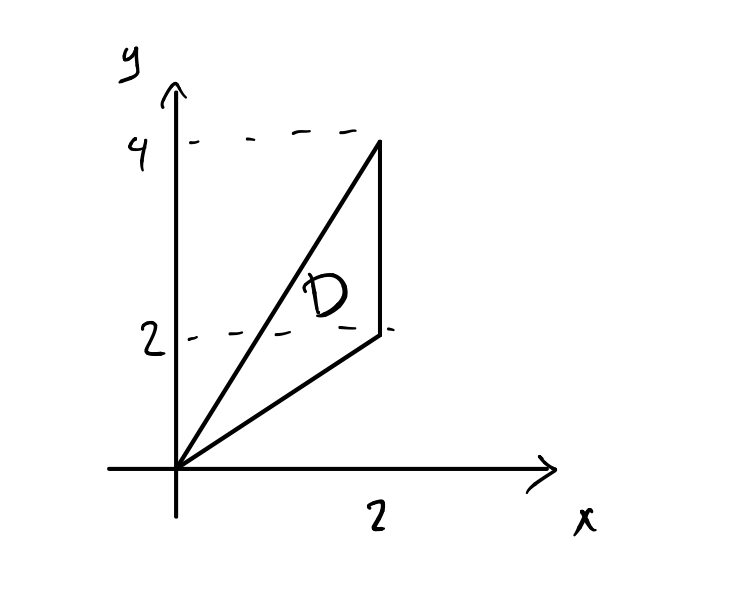
\includegraphics[scale=.3]{example.jpeg}
\end{figure}


Normally we'd write 3 line integrals, one for each edge of the triangle. However, by Green's theorem, \begin{align*}
\int_c xy^2dx +2x^2 y dy=&\iint_D \frac{\p}{\p x}(2x^2y)-\py (xy^2) dA\\
=&\int_0^2\int_x^{2x } 4xy-2xydy dx\\
=&12,
\end{align*} and this is quite a faster way to do this.
\end{solution}

\textbf{Fun fact:} You can use Green's theorem to show equality of mixed partials for twice continuously differnetiable functions in a couple of lines! Let $f$ be such a function, and let $\vF=\nabla f=\lg P,Q\rg$. Then, by Green's theorem, for any small disk $D$, $$\iint \left( \Q-\P\right )dA=\iint_D \frac{\p^2 f}{\p x\p y}-\frac{\p^2 f}{\p y\p x}dA=\int_c\nabla f \cdot d\vr=0,$$ by FTC. This shows that $\frac{\p^2 f}{\p y\p x}=\frac{\p^2f}{\p x\p y}$ everywhere.

\subsubsection*{Green's theorem for calculating areas}
We can use Green's Theorem to express the area of a domain. If we set $Q=x$, $P=0$ we find \begin{equation}
\int_c x dy=\iint_D 1 dA =A(D)
\end{equation}
and by setting $P=-y$, $Q=0$, \begin{equation}
\int_c -y dx=\iint_D 1 dA =A(D)
\end{equation}
\begin{example}
Find the area enclosed by the ellipse $$\frac{x^2}{a^2}+\frac{y^2}{b^2}=1.$$ 
\end{example}
\begin{solution}
This is an exercise you might have done in math 125, where you used trigonometric substitution. Here we'll do it using Green's theorem. We parametrize the ellipse by \begin{align}
x(t)=&a\cos(t)\\
y(t)=&b\sin(t),
\end{align}
for $t\in[a,b]$. Then \begin{align*}
Area=&\iint_D 1 dA\\
=&\int_0^{2\pi}x(t)y'(t) dt\\
=&\int_0^{2\pi}a\cos(t)b\sin(t)dt\\
=&\pi a b.
\end{align*}
\end{solution}


\subsubsection*{${}^*$Using Green's theorem to transfer a computation of a line integral to a line integral over a more convenient curve}
For this example, we'll use the vector field $\vF(x,y)=\lg \frac{-y}{x^2+y^2},\frac{x}{x^2+y^2}\rg=\lg P(x,y),Q(x,y)\rg$, defined on $\R^2\backslash \{(0,0)\}$. Suppose we want to find its line integral over the ellipse $\frac{x^2}{a^2}+\frac{y^2}{b^2}=1,$ positively oriented (in fact, any simple closed curve, but let's stick with the ellipse for now). Explicitly calculating this is possible, but not straightforward, so we'll see another way to do it.


You might remember from the last section that $\P-\Q=0$ everywhere on $D$. Note that \textbf{we can't use Green's theorem}, because $\P$ and $\Q$ are not continuous inside the ellipse (they blow up at 0). Here's what we'll do instead. We create 2 simple closed curves where we can indeed apply Green's Theorem, as in the picture, by inserting a small circle of radius $\e $ about the origin and connecting it to the ellipse.

\begin{figure}[h]
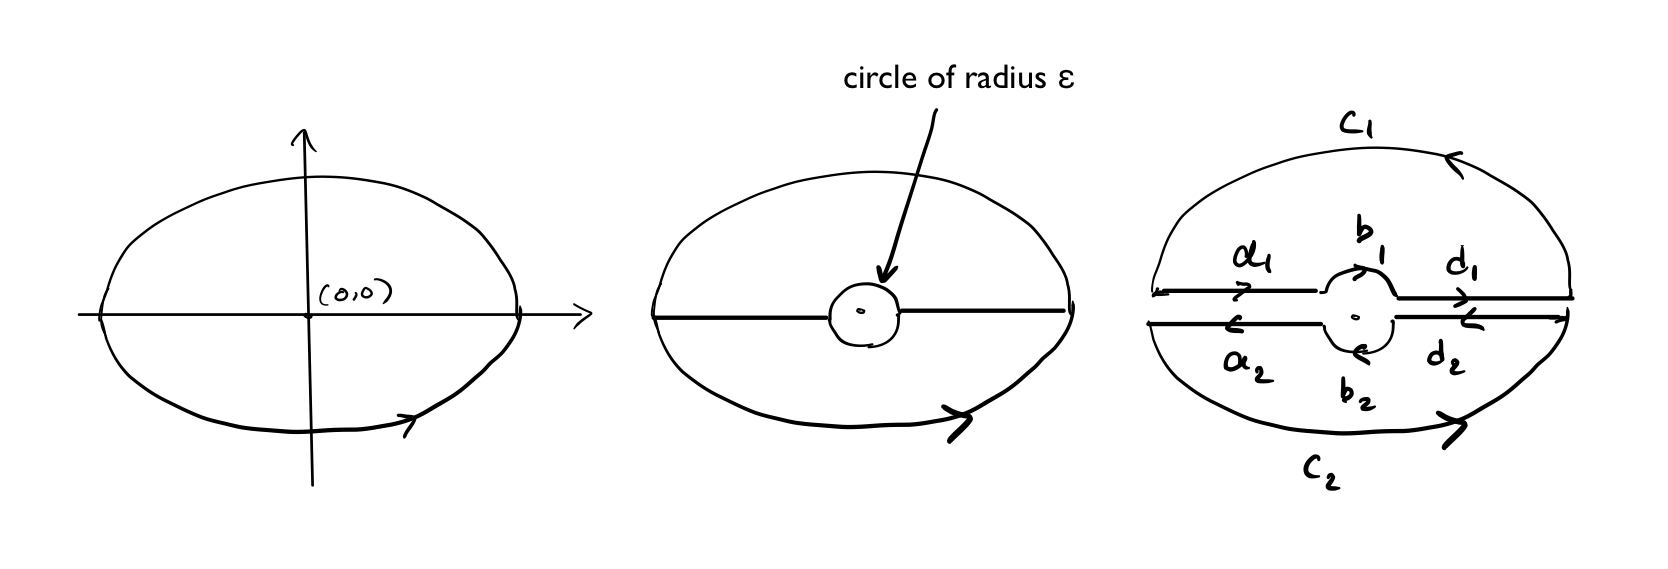
\includegraphics[scale=.3]{last.jpg}
\end{figure}


Note that in the picture \begin{align*}
&c= c_1\cup c_2\\
&a_1=-a_2\\
&d_1=-d_2
\end{align*}

We may apply Green's Theorem in $D_1$ and $D_2$ because $\P$ and $\Q$ \textbf{are} continuous there, and  $\Q-\P=0$ in both of those sets. Therefore,
\begin{equation}
\label{eqn1} 0=\iint_{D_1}\Q-\P dA=\int_{c_1}\vF\cdot d\vr+\int_{a_1}\Fline +\int_{b_1}\Fline+\int_{d_1}\Fline
\end{equation}
and \begin{equation}
\label{eqn2} 0=\iint_{D_2}\Q-\P dA=\int_{c_2}\vF\cdot d\vr+\int_{a_2}\Fline +\int_{b_2}\Fline+\int_{d_2}\Fline.
\end{equation}
Adding \eqref{eqn1} and \eqref{eqn2}, we find \begin{align*}
0=\left (\int_{c_1}\vF\cdot d\vr+\int_{c_2}\vF\cdot d\vr\right )&+\left (\int_{a_1}\Fline +\int_{a_2}\Fline\right )\\&+\left (\int_{b_1}\Fline+\int_{b_2}\Fline\right )+\left (\int_{d_1}\Fline+\int_{d_2}\Fline\right ).
\end{align*}
and this gives, using that $a_1=-a_2$ and $d_a=-d_2$, $$\int_c\Fline=\int_b\Fline,$$ where $b$ is the circle of radius $\e$, positively oriented.

Now we parametrize $b$ by $x(t)=\e\cos(t)$, $y(t)=\e\sin(t)$, $t\in [0,\pi]$ and find $$\int_c\Fline =\int_0^{2\pi}\lg\frac{-\e \sin(t)}{\e^2},\frac{\e\cos(t)}{\e^2}\rg\cdot\lg -\e\sin(t),\e\cos(t)\rg dt=\dots=2\pi.$$
(check!). It is quite remarkable in a sense that $\e$ does not appear at the end, but also expected, since there is no $\e$ in the integral over the ellipse that we want to compute!


\end{document}

